\chapter{Results and Discussion} % Main chapter title

\label{Chapter5} % Change X to a consecutive number; for referencing this chapter elsewhere, use \ref{ChapterX}

\section{Phenanthrene parameterization}

The first part of this work consisted in obtaining phenanthrene parameters for the SAFT-$\gamma$ Mie Force Field as described in Section \ref{parame}. This part was necessary since these parameters were not available for the ring geometry on the force field database \cite{ervik2016}. We carried out this parameterization using the free energy of Helmholtz equations for rings of \cite{lafitte2012}, Eq. \ref{eqn:aringlafitte}, and of \cite{muller2017}, Eq. \ref{eqn:aringmuller}. The parameters obtained with these two strategies and the mean percentage error (MPE) to the experimental data \cite{pvphen,osborn} were those observed in Table \ref{tbl:estimparameters}.

\begin{table}[h]
	\centering
	\caption{Estimated SAFT-$\gamma$ Mie force field parameters for phenanthrene.}
	\label{tbl:estimparameters}
	\begin{tabular}{ccccc}
		\hline\hline
		$m_s$                & $\epsilon/\kappa_{b}$ (K) & $\sigma$ (\AA) & $\lambda_r$ & MPE(\%)   \\ \hline\hline
		3 \cite{lafitte2012} & 485.55               & 4.197              & 14.34       & 1.48|9.74 \\
		5  \cite{muller2017} & 262.74               & 4.077              & 9.55        & 0.88      \\ \hline\hline
	\end{tabular}
	
\end{table} 

The MPE value of 1.64 for the \citeonline{lafitte2012} strategy in the Table \ref{tbl:estimparameters} is the error between the vapor pressure calculated with the equation of state and the experimental data. The second MPE value for the \citeonline{lafitte2012} strategy (9.74) is the error between the vapor pressure calculated with the equation of state and the vapor pressure obtained in the GEMC simulations. We also show, in Figure \ref{fig:fitede}, the vapor pressure curve obtained using the EoS with the two free energy of Helmholtz equations for rings. It's clear, observing the figure mentioned above and the MPE     values for both equations for rings, that both approaches for the EoS performed very similar and were able to reproduce the experimental data. However, the parameters estimated with the equation of \citeonline{lafitte2012}  could not be directly transferred to molecular simulations because this strategy needs an estimation with molecular simulation. This additional procedure is not necessary when estimating parameters for the chain equation \cite{avendano2011} or the ring equation of \citeonline{muller2017}. In addition to that, this use of molecular simulation data to acquire the parameters negates the overall idea proposed by \cite{avendano2011}. They developed this force field with the intention of obtaining the parameters in a more straightforward way than other force fields since the SAFT-$\gamma$ Mie model would not have the computational time associated with doing molecular simulations in its parameterization. Due to these specific characteristics of the model of \citeonline{lafitte2012}, we only studied the solvation free energy of phenanthrene with the set of parameters estimated with the strategy of \citeonline{muller2017}. In fact, we only followed the approach of \citeonline{lafitte2012} because it was the only one available when we first started this research. The sets of parameters and geometries for the other compounds were retrieved from the literature, and they are exposed in Tables \ref{tbl:parameters} and \ref{tbl:geopara}.

\begin{figure}[h]
	\centering
	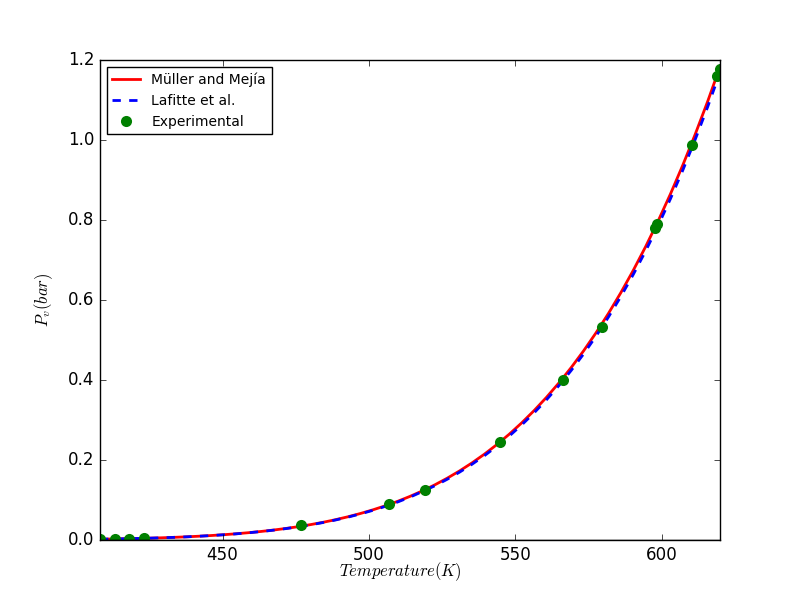
\includegraphics[width=0.8\linewidth]{Figures/ede}
	\caption{Vapor pressure ($P_{v}$) of phenanthrene calculated with the two strategies of the SAFT-VR Mie EoS for modeling molecules formed by rings.} 
	\label{fig:fitede}
\end{figure}

\section{Solvation free energies}
Our primary intention with this study is to assess the capability of the SAFT-$\gamma$ Mie force field to represent solvation free energies. Hence, we chose benchmark solutes used in the literature (benzene, propane) and polyaromatic solutes (benzene, pyrene, phenanthrene, anthracene), and, for the solvents, we picked non-polar (hexane), aromatic (toluene), and hydrogen bonding (1-octanol, water) substances. It would be interesting to do a study with a bigger database of pairs solvent-solute. However, the time required for performing each of the solvation free energy simulations, some difficulties related to the available computational structure, and the fact that a better model of aromatic compounds with this force field was only published in the middle of our study prevented us from doing a more extensive study. The solvation free energy simulations for the pairs chosen were carried out with binary interaction parameters equal to zero since these parameters were not necessary according to our preliminary studies. Since the force field does not account for charges, we only calculated the Mie contribution (Eq. \eqref{eq:softcore}) to the solvation free energy. A total of 15 to 18 $\lambda 's$, depending on the solute-solvent pairs, and their respective $\eta 's$ were estimated as described in Sections \ref{ee} and \ref{solvme}. The simulations carried out using these optimized weights deviated from the flat-histogram requirement of equal number visits by an average of 5\% for all of the pairs solvent+solute. The final $\lambda$ set for all the pairs was found using the cumulative probability distribution (Eq. \eqref{eqn:cumfun}). The probability distribution for the hexane(solvent)+benzene(solute) pair can be seen in \figref{fig:optimized_cdf}. From now on we are going to use the terminology solvent+solute. The optimized values of $\lambda$ and $\eta$ for this pair and all the other pairs are available in Tables \ref{tbl:lambdahex} to \ref{tbl:lambdaco2}. By observing the coupling parameters found for all the pairs, we can see that they are concentrated on the region with a steeper slope as it is expected in this method.

\begin{figure}[h]
	\centering
	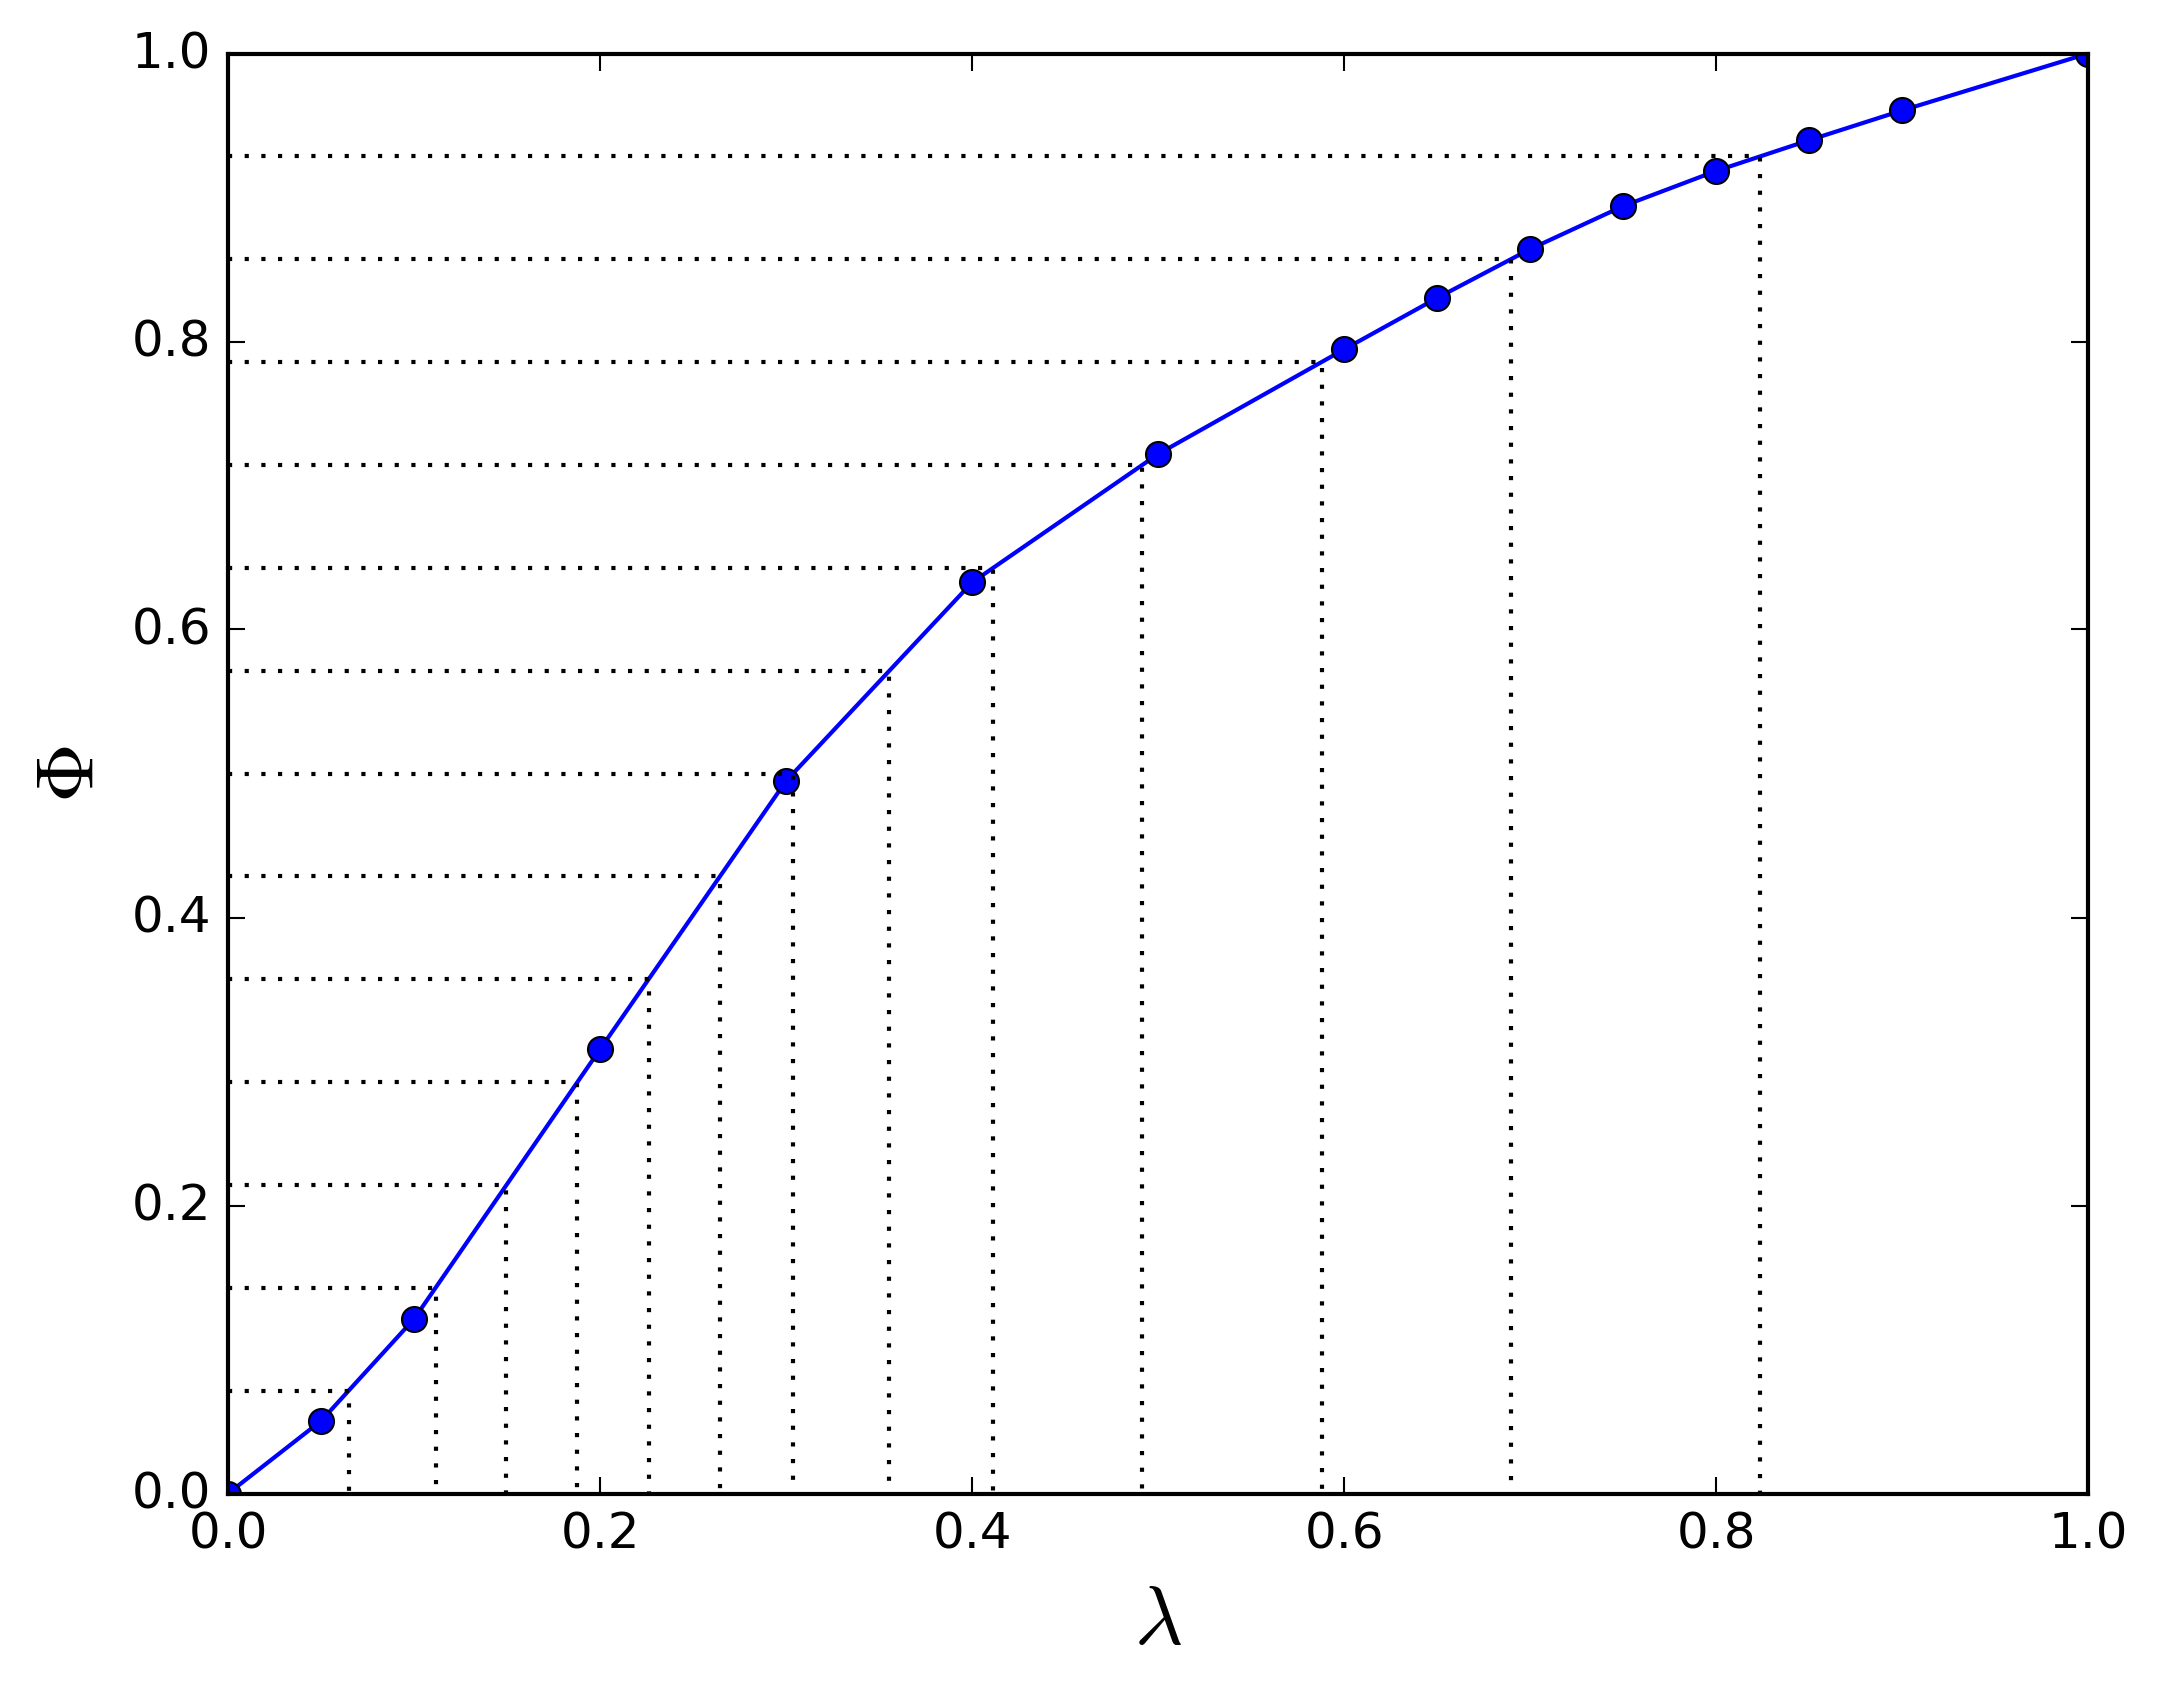
\includegraphics[width=0.72\linewidth]{Figures/optimized_cdf}
	\caption{Cumulative probability used to obtain the optimized values of $\lambda 's$ for the pair hexane+benzene.}
	\label{fig:optimized_cdf}
\end{figure}

%Simulations using these weights deviated
%by an average of 5% from flat histogram occupancy
%in states, with an average maximum deviation over all
%simulations of less than 10%.

\begin{table}[h]
	\centering
	\caption{Optimized values of $\lambda $ and $\eta $ for the hexane+solute pairs.}
	\label{tbl:lambdahex}
	\begin{tabular}{cccccc}
		\hline\hline
		\multicolumn{2}{c}{benzene}&\multicolumn{2}{c}{pyrene}& \multicolumn{2}{c}{phenanthrene}\\
		\hline\hline
		$\lambda$ & $\eta$& $\lambda$ & $\eta$  & $\lambda$ & $\eta$   \\ 
		\hline\hline
		0.000     &0.000      & 0.000    &    0.000    &    0.000    &    0.000    \\
		0.065     &0.708  & 0.076    &    4.234    &    0.090    &    1.981    \\
		0.112     &1.385  & 0.107    &    5.620    &    0.132    &    3.461    \\
		0.15      &1.892  & 0.132    &    6.499    &    0.161    &    4.494    \\
		0.188     &2.399  & 0.152    &    6.690    &    0.185    &    5.185    \\
		0.226     &2.519  & 0.170    &    6.643    &    0.205    &    5.552    \\
		0.264     &2.457  & 0.189    &    6.461    &    0.224    &    5.725    \\
		0.304     &2.367  & 0.213    &    6.091    &    0.244    &    5.722    \\
		0.356     &1.921  & 0.242    &    5.566    &    0.268    &    5.523    \\
		0.411     &1.411  & 0.280    &    4.729    &    0.305    &    4.975    \\
		0.492     &0.524  & 0.355    &    2.853    &    0.372    &    3.576    \\
		0.588     &-0.663 & 0.483    &    -0.778    &    0.500    &    0.297    \\
		0.69      &-2.016 & 0.678    &    -6.947    &    0.560    &    -1.390    \\
		0.824     &-3.922 & 0.788    &    -10.631    &    0.722    &    -6.309    \\
		1.000         &-6.583  &1.000      &    -18.141    &    1.000    &    -15.448    \\
		\hline\hline   
	\end{tabular}
\end{table}
\begin{table}[h]
	\centering
	\caption{Optimized values of $\lambda $ and $\eta$ for the 1-octanol+solute pairs.}
	\begin{tabular}{cccccc}
		\hline\hline
		\multicolumn{2}{c}{propane}& \multicolumn{2}{c}{anthracene}& \multicolumn{2}{c}{phenanthrene}\\
		\hline\hline
		$\lambda$ & $\eta$ & $\lambda$ & $\eta$  & $\lambda$ & $\eta$   \\ 
		\hline\hline
		0.000    &    0.000    &    0.000    &    0.000    &    0.000    &    0.000    \\
		0.027    &    3.126    &    0.078    &    3.932    &    0.049    &    2.578    \\
		0.050    &    5.109    &    0.111    &    6.178    &    0.091    &    5.663    \\
		0.073    &    6.093    &    0.130    &    7.426    &    0.125    &    8.575    \\
		0.095    &    6.570    &    0.143    &    8.201    &    0.144    &    10.069    \\
		0.117    &    6.826    &    0.154    &    8.717    &    0.157    &    10.978    \\
		0.142    &    6.956    &    0.164    &    9.085    &    0.169    &    11.599    \\
		0.174    &    6.969    &    0.174    &    9.357    &    0.180    &    12.040    \\
		0.215    &    6.847    &    0.184    &    9.556    &    0.192    &    12.340    \\
		0.269    &    6.554    &    0.197    &    9.676    &    0.206    &    12.499    \\
		0.337    &    6.050    &    0.214    &    9.681    &    0.225    &    12.478    \\
		0.427    &    5.228    &    0.238    &    9.490    &    0.253    &    12.161    \\
		0.545    &    3.955    &    0.274    &    8.958    &    0.298    &    11.280    \\
		0.720    &    1.843    &    0.326    &    7.906    &    0.371    &    9.406    \\
		1.000    &    -1.903    &    0.399    &    6.088    &    0.484    &    5.891    \\
		&        &    0.515    &    2.777    &    0.664    &    -0.516    \\
		&        &    0.695    &    -2.960    &    0.802    &    -5.908    \\
		&        &    1.000    &    -13.768    &    1.000    &    -14.073    \\
		\hline\hline
	\end{tabular}
\end{table}
\begin{table}[h]
	\centering
	\caption{Optimized values of $\lambda $ and $\eta$ for the toluene+solute pairs.}
	\begin{tabular}{cccccc}
		\hline\hline
		\multicolumn{2}{c}{pyrene}& \multicolumn{2}{c}{anthracene}& \multicolumn{2}{c}{phenanthrene}\\
		\hline\hline
		$\lambda$ & $\eta$ & $\lambda$ & $\eta$  & $\lambda$ & $\eta$   \\ 
		\hline\hline
		0.000    &    0.000    &    0.000    &    0.000    &    0.000    &    0.000    \\
		0.090    &    2.563    &    0.119    &    0.218    &    0.136    &    0.726    \\
		0.130    &    4.338    &    0.174    &    1.210    &    0.191    &    2.307    \\
		0.154    &    5.439    &    0.209    &    2.052    &    0.223    &    3.430    \\
		0.172    &    6.181    &    0.236    &    2.664    &    0.246    &    4.233    \\
		0.188    &    6.670    &    0.261    &    3.122    &    0.264    &    4.780    \\
		0.204    &    6.986    &    0.283    &    3.378    &    0.281    &    5.149    \\
		0.222    &    7.121    &    0.306    &    3.449    &    0.299    &    5.354    \\
		0.244    &    7.025    &    0.332    &    3.311    &    0.318    &    5.389    \\
		0.278    &    6.520    &    0.360    &    2.936    &    0.340    &    5.222    \\
		0.340    &    5.010    &    0.399    &    2.209    &    0.372    &    4.717    \\
		0.462    &    1.247    &    0.466    &    0.567    &    0.425    &    3.440    \\
		0.616    &    -4.283    &    0.564    &    -2.211    &    0.524    &    0.444    \\
		0.788    &    -11.032    &    0.715    &    -6.983    &    0.701    &    -5.814    \\
		1.000    &    -19.814    &    1.000    &    -16.923    &    1.000    &    -17.803    \\        
		\hline\hline
	\end{tabular}
\end{table}

\begin{table}[h]
	\centering
	\caption{Optimized values of $\lambda $ and $\eta $ for the phenanthrene+$CO_{2}$+ toluene mixture with different values of $w_{CO_{2}}$.}
	\label{tbl:lambdaco2}
	\begin{tabular}{cccccccc}
		\hline\hline
		\multicolumn{2}{c}{$w_{CO_{2}}=0.087$}& \multicolumn{2}{c}{$w_{CO_{2}}=0.119$}& \multicolumn{2}{c}{$w_{CO_{2}}=0.169$}& \multicolumn{2}{c}{$w_{CO_{2}}=0.289$}\\
		\hline\hline
		$\lambda$ & $\eta$ & $\lambda$ & $\eta$  & $\lambda$ & $\eta$  & $\lambda$ & $\eta$ \\ 
		\hline\hline
		0.000    &    0.000    &    0.000    &    0.000    &    0.000    &    0.000    &    0.000    &    0.000    \\
		0.128    &    0.604    &    0.128    &    0.732    &    0.064    &    0.883    &    0.066    &    0.806    \\
		0.184    &    2.067    &    0.186    &    2.223    &    0.108    &    0.764    &    0.111    &    0.760    \\
		0.217    &    3.164    &    0.219    &    3.319    &    0.175    &    1.969    &    0.172    &    1.983    \\
		0.240    &    3.940    &    0.244    &    4.098    &    0.214    &    3.156    &    0.204    &    2.967    \\
		0.260    &    4.472    &    0.267    &    4.704    &    0.240    &    3.974    &    0.227    &    3.627    \\
		0.277    &    4.823    &    0.289    &    5.031    &    0.258    &    4.457    &    0.245    &    4.082    \\
		0.295    &    5.035    &    0.313    &    5.084    &    0.273    &    4.750    &    0.262    &    4.395    \\
		0.318    &    5.059    &    0.339    &    4.950    &    0.287    &    4.921    &    0.279    &    4.583    \\
		0.347    &    4.762    &    0.373    &    4.371    &    0.305    &    4.962    &    0.299    &    4.621    \\
		0.397    &    3.753    &    0.425    &    3.055    &    0.326    &    4.885    &    0.325    &    4.423    \\
		0.491    &    1.031    &    0.488    &    1.196    &    0.361    &    4.401    &    0.365    &    3.739    \\
		0.670    &    -5.148    &    0.525    &    -0.027    &    0.419    &    2.990    &    0.428    &    2.198    \\
		0.791    &    -9.713    &    0.730    &    -7.185    &    0.527    &    -0.299    &    0.530    &    -0.842    \\
		1.000    &    -18.098    &    1.000    &    -17.769    &    0.697    &    -6.180    &    0.701    &    -6.763    \\
		&        &        &        &    1.000    &    -17.998    &    1.000    &    -18.163    \\
		\hline\hline
	\end{tabular}
\end{table}
\FloatBarrier
It is also essential to analyze the reliability of solvation free energy estimations through the overlapping of the intermediate states. Insufficient overlap among states when using FEP based methods such as MBAR may result in the underestimation of variance and, consequently, in substantially incorrect solvation free energies \cite{klimovich}. The overlap matrix for the solvation free energy of benzene in hexane is presented in \figref{fig:hexove} and the matrices for the other pairs are available in Appendix \ref{overlapmatrix}. Each element $ij$ of these matrices is the average probability of observing a configuration sampled from state i in state j. As an example, the average probability of finding a configuration sampled from state 3 in state 4 is 0.11 in \figref{fig:hexove}. According to \citeonline{klimovich}, a tridiagonal overlap matrix is an indication of reliable free energy estimates, as long as the resulting error is sufficiently low. They define a tridiagonal matrix as one matrix with elements appreciably different from zero (the values should be as low as 0.03) in the main diagonal and the first diagonals above and below the main one. This requirement was met for all the pairs in our study. Some of the overlap matrices, including the one in Figure \ref{fig:hexove}, had more than three diagonals, and, consequently, an apparent unnecessary number of intermediate states. However, this number of intermediate states was indispensable in our study because the error estimate of the solvation free energies significantly increased when we removed some of the intermediate states. Hence, we maintained these intermediate states in order to obtain low error values. After this analysis, we present in Table \ref{tbl:solv1} the results for solvation free energy calculations, the errors from these estimations with MBAR, and the absolute deviations from experimental data \cite{doi:10.1021/ci034120c}.  

\begin{figure}[h]
	\centering
	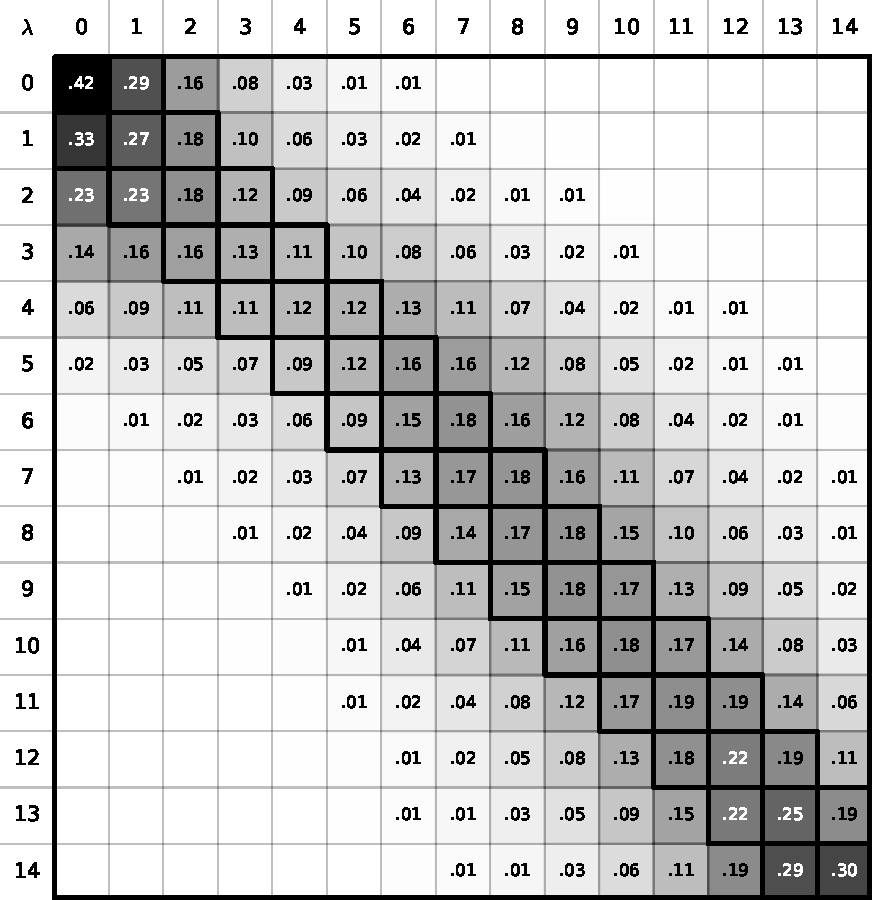
\includegraphics[width=0.7\textwidth]{Figures/ohex_benz}
	\caption{Overlap matrix for hexane+benzene.}
	\label{fig:hexove}
\end{figure}

\begin{table}[h]
	\centering
	\caption{Calculated and experimental values for the solvation free energies (kcal/mol) of solutes in non-aqueous solvents.}
	\label{tbl:solv1}
	\begin{tabular}{cccccc}
		\hline\hline
		Solute       & Solvent   & $\Delta G_{solv}^{exp}$ & $\Delta G_{solv}^{Mie}$ & Absolute  &  \\
		&           &                         &                         & Deviation &  \\ \hline\hline
		benzene      & hexane    & -3.96                   & -3.76  $\,$ $\pm$ 0.01       & 0.20      &  \\
		pyrene       & hexane    & -11.53                  & -10.82 $\pm$ 0.02       & 0.71      &  \\
		phenanthrene & hexane    & -10.01                  & -9.16  $\,$ $\pm$ 0.01       & 0.85      &  \\
		propane      & 1-octanol & -1.32                   & -1.36  $\,$ $\pm$ 0.03       & 0.04      &  \\
		anthracene   & 1-octanol & -11.72                  & -8.12   $\,$ $\pm$ 0.03       & 3.61      &  \\
		phenanthrene & 1-octanol & -10.22                  & -8.34  $\,$ $\pm$ 0.03       & 1.47      &  \\
		pyrene       & toluene   & -12.86                  & -11.74 $\pm$ 0.01       & 1.11      &  \\
		anthracene   & toluene   & -11.31                  & -9.90 $\,$ $\pm$ 0.01        & 1.41      &  \\ \hline\hline
		&
	\end{tabular}
\end{table}
\FloatBarrier

The numerical values for solvation free energies in hexane had overall smaller absolute deviations from experimental data than the deviations in the other solvents. Additionally, this force field presented better results for the pair hexane+benzene than the TraPPE force field (- 4.35  $\pm$ 0.05 kcal/mol) \cite{garrido2011} and the ELBA coarse-grained force field  (-2.92 $\pm$ 0.01 kcal/mol) \cite{doi:10.1021/acs.jctc.5b00963}. TraPPE is a force field parametrized with fluid-phase equilibria data that uses the Lennard-Jones potential to describe the non-bonded interactions. In the cited paper, they used the united-atom description of the TraPPE force field for the alkyl group, the all-atom description for the polar groups and the explicit-hydrogen approach for the aromatic groups. In the explicit-hydrogen approach, the interaction sites for all hydrogen atoms, some lone pair electrons, and bond centers are accounted for \cite{doi:10.1021/jp073586l}. In turn, the ELBA force field is a coarse-grained model that comprises six independent parameters. This force field models three carbons as one Lennard-Jones site and one water molecule as a single Lennard-Jones site with a point dipole. We also present the solvation free energies corresponding to each alchemical state ($\lambda$) for all the pairs studied here in Figures \ref{fig:hex} to \ref{fig:tol}. In these figures, we did not represent the errors of the estimation with MBAR because they were too small to be seen. Specifically observing the solvation free energy in hexane (Figure \ref{fig:hex}), we can see the effect of the molecule's size on the entropic region of the free energy curve. This region corresponds to the first values of $\lambda$ where space in the solvent is being 'opened' for the insertion of the solute.

We expected that a force field based on an EoS that does not explicitly account for hydrogen bond would not perform well for 1-octanol in mixtures since the parameterization of this molecule did not explicitly account for the interactions of association. All the beads representing 1-octanol have the same intermolecular parameter, and there is no distinction between the polar and apolar groups. Despite this, the solvation free energies of propane and phenanthrene in 1-octanol lied in the desired deviation range of 1-2 kcal/mol \cite{doimobley}. For propane, the observed deviation in solvation free energies was much smaller when compared to the other solutes, which can be attributed to the non-polarity of propane and its smoother free energy curve, presented in Figure \ref{fig:oct}. Such solvation free energy of propane in 1-octanol also had a smaller deviation than the prediction of the ELBA force field (-0.92 $\pm$ 0.01) \cite{doi:10.1021/acs.jctc.5b00963}. The absolute deviation of the solvation free energy computed for anthracene in 1-octanol is much higher than the one calculated for phenanthrene in 1-octanol. The anthracene and phenanthrene molecules have the same geometry (Figure \ref{fig:fen5}) in the SAFT-$\gamma$ Mie model, although anthracene is a linear molecule and phenanthrene is not, and also similar physical properties. Hence, this high deviation of the solvation free energy of anthracene in 1-octanol may indicate a problem in the geometry chosen for anthracene in the SAFT-$\gamma$ Mie force field and the importance of the geometry in modeling the molecules with this force field.      
\FloatBarrier
\begin{figure}[H]
	\centering
	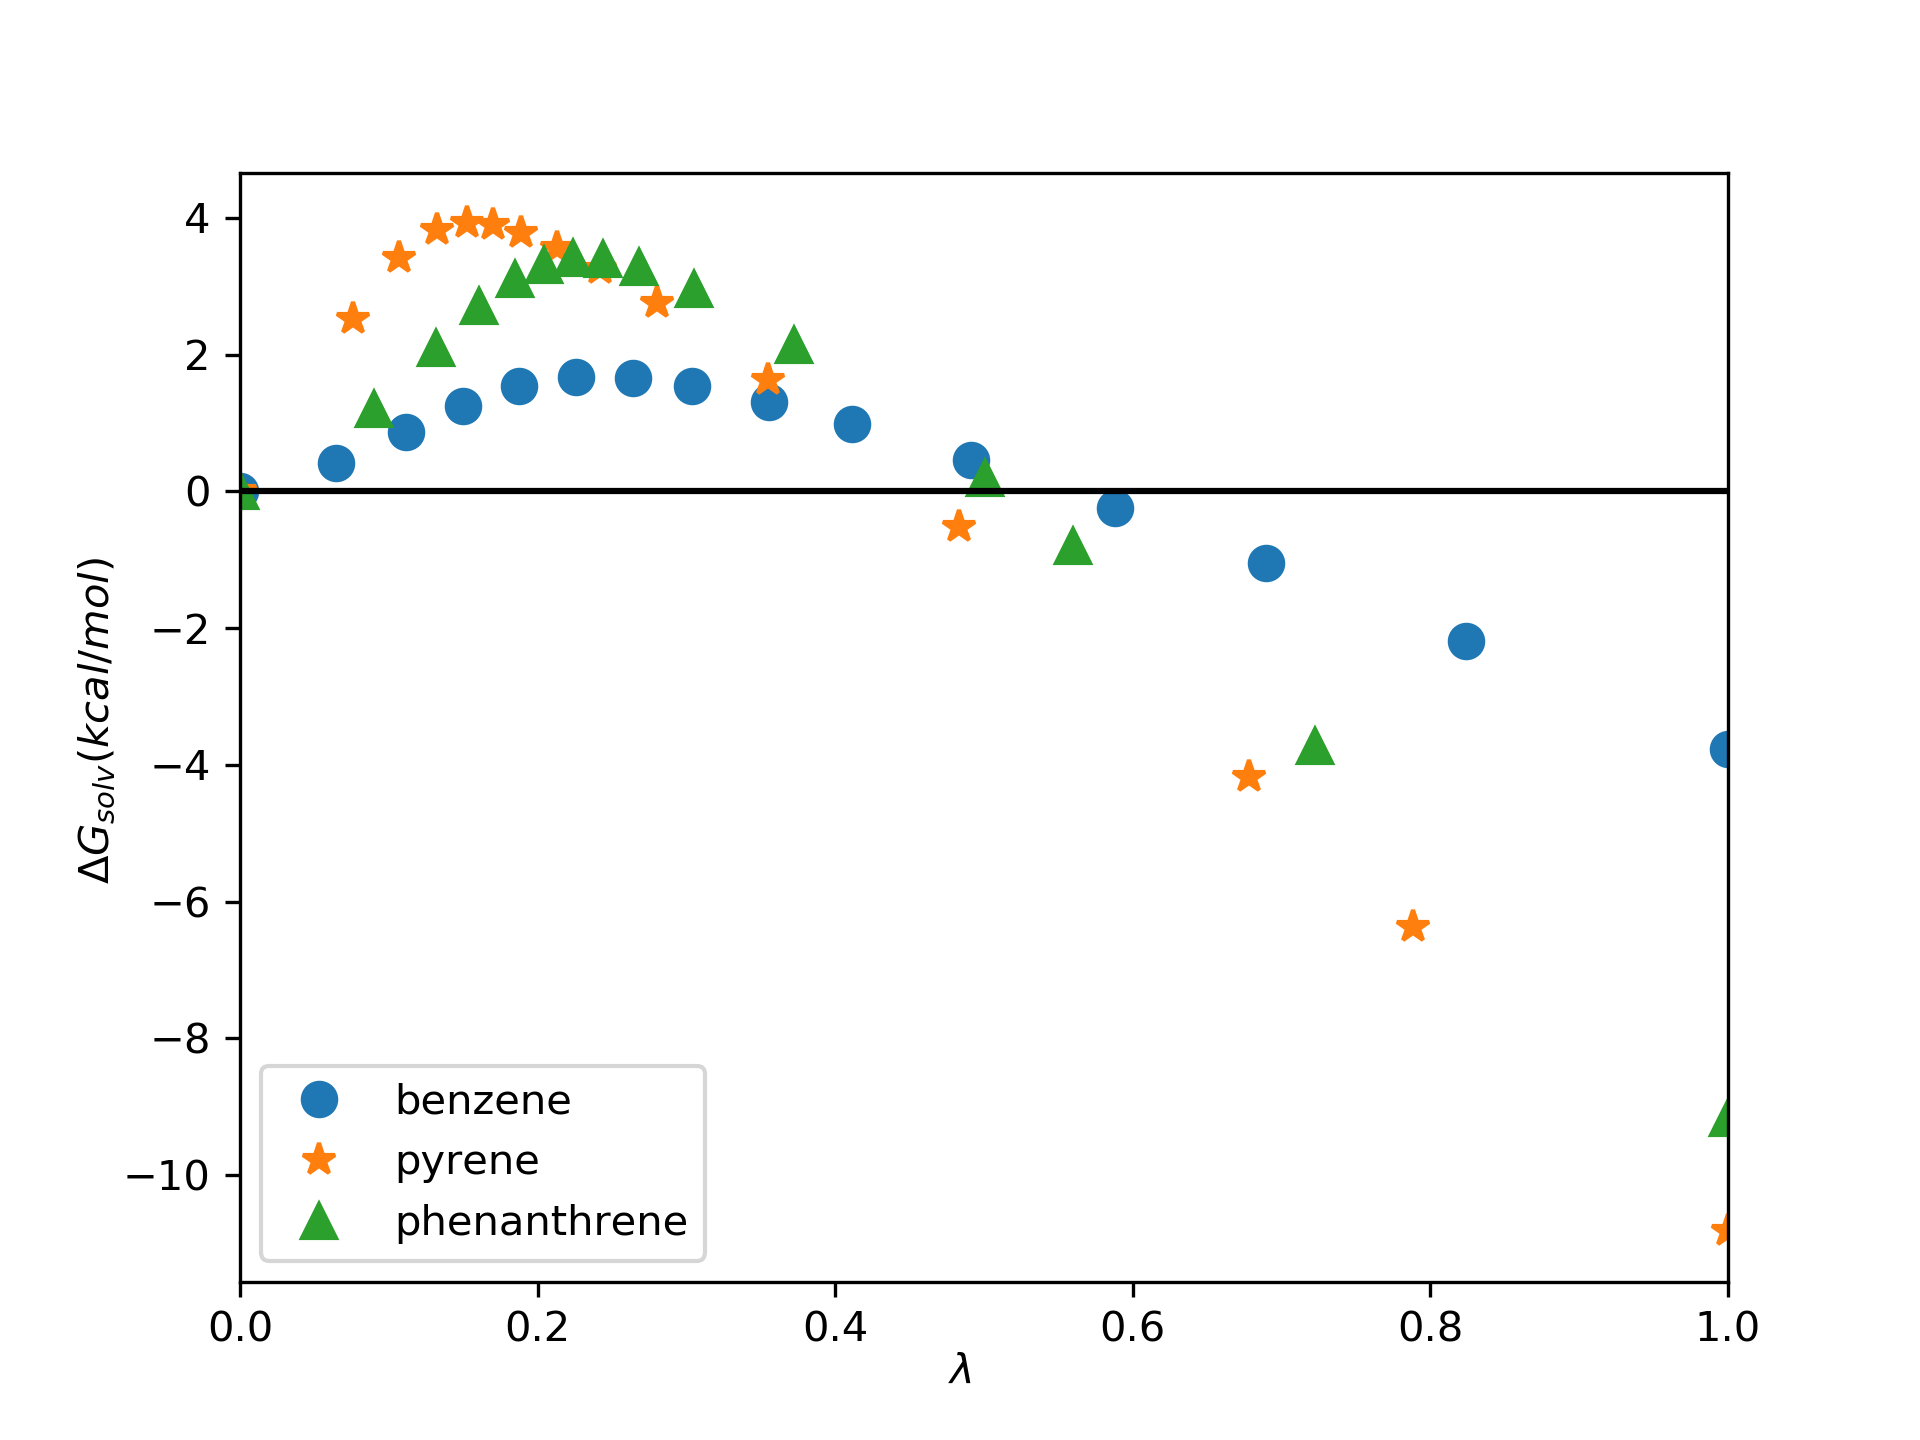
\includegraphics[width=0.8\textwidth]{Figures/hex}
	\caption{Representation of solvation free energies of different solutes in hexane corresponding to each alchemical state.}
	\label{fig:hex}
\end{figure}

\begin{figure}[H]
	\centering
	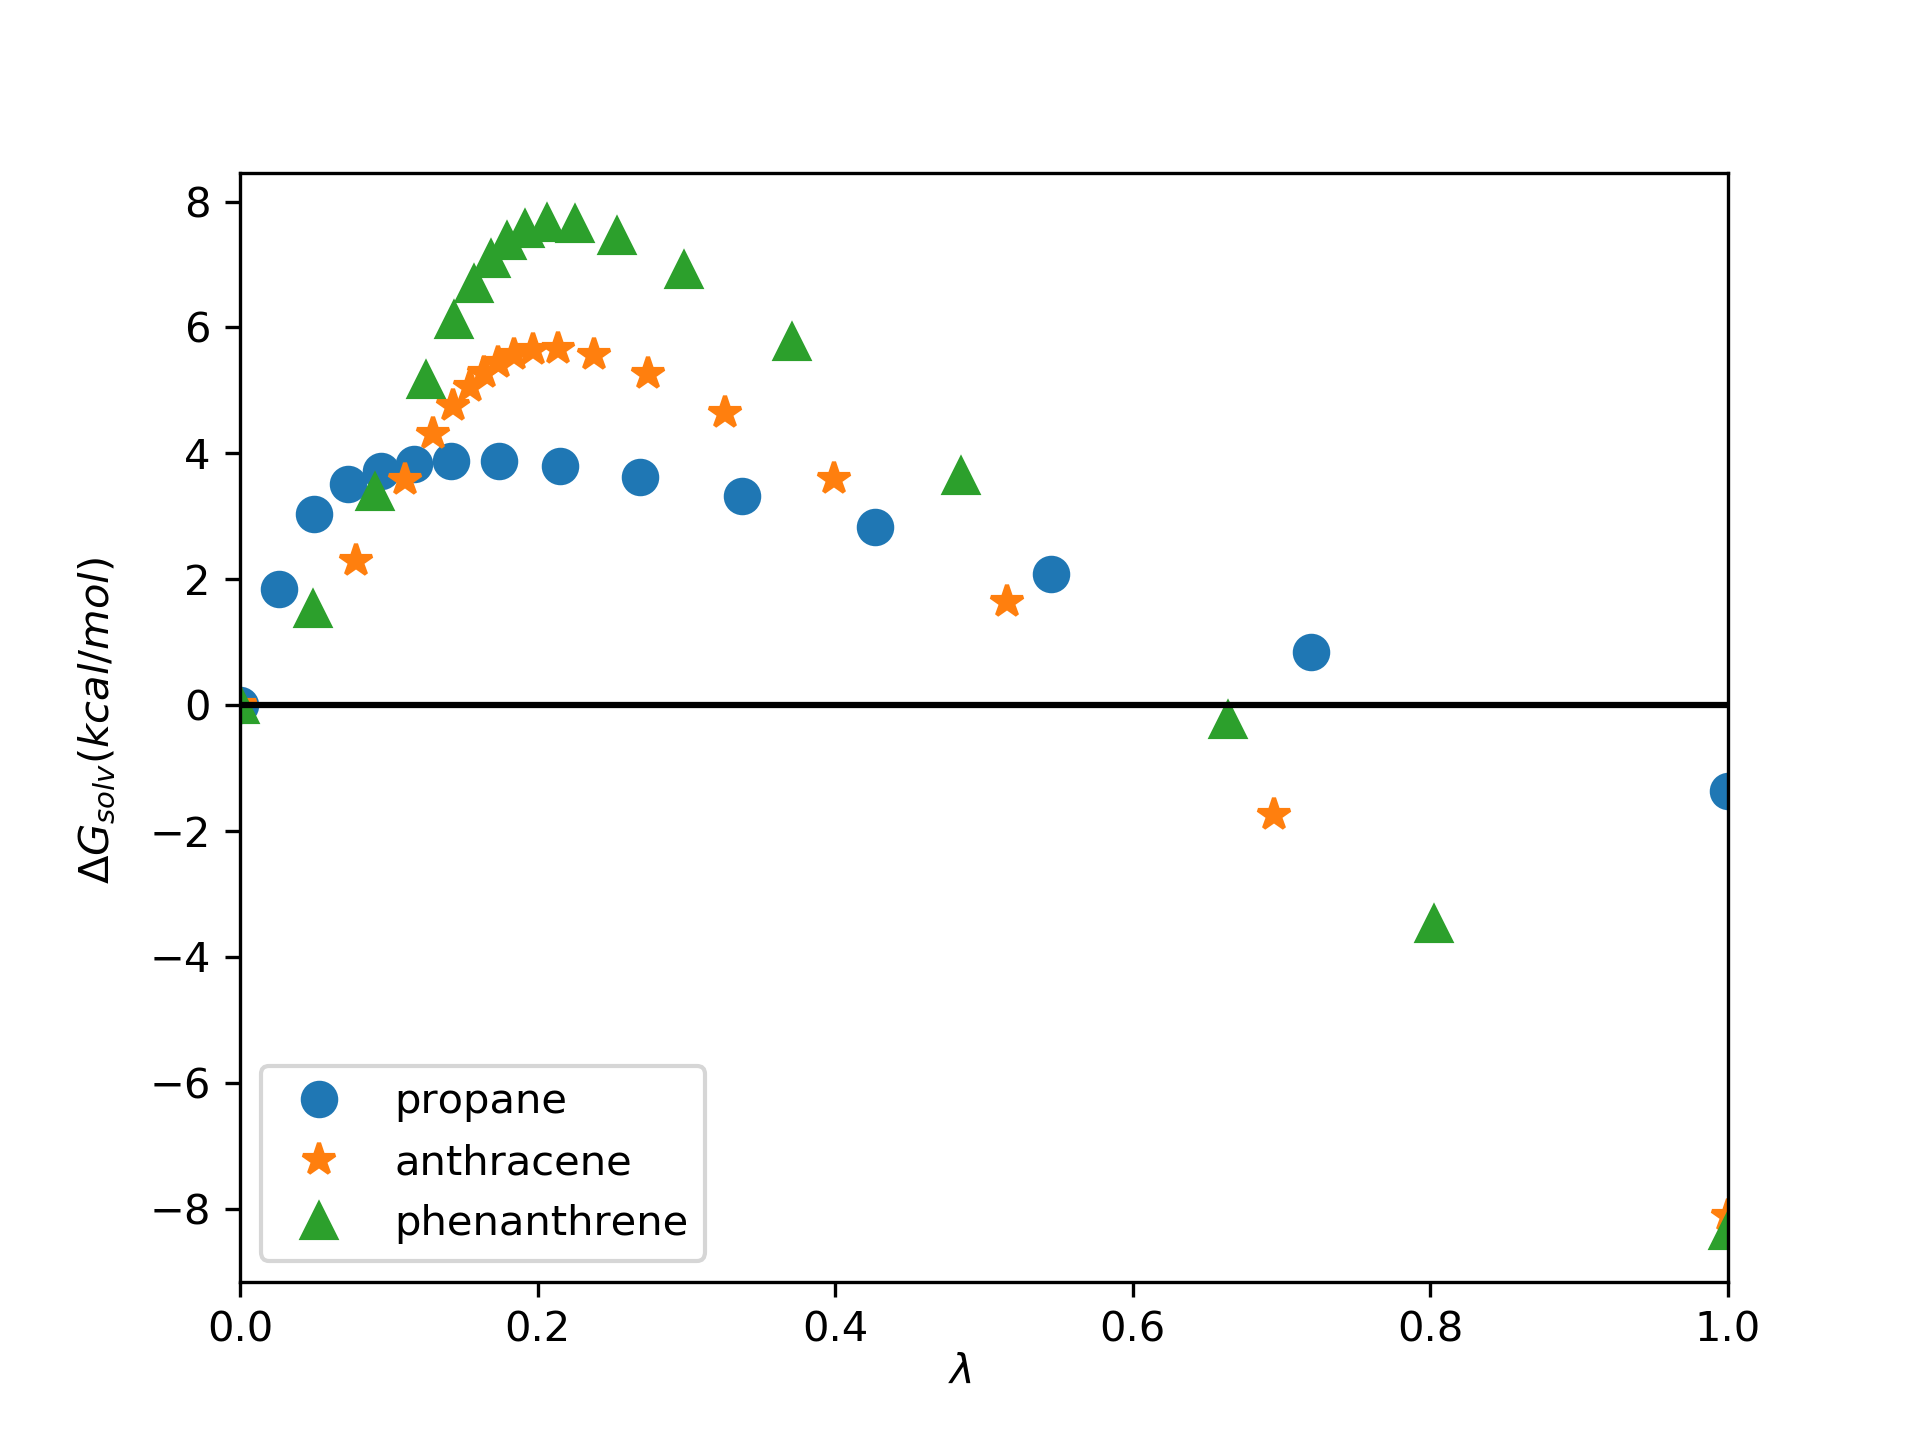
\includegraphics[width=0.8\textwidth]{Figures/oct}
	\caption{Representation of solvation free energies of different solutes in 1-octanol corresponding to each alchemical state.}
	\label{fig:oct}
\end{figure}

\begin{figure}[H]
	\centering
	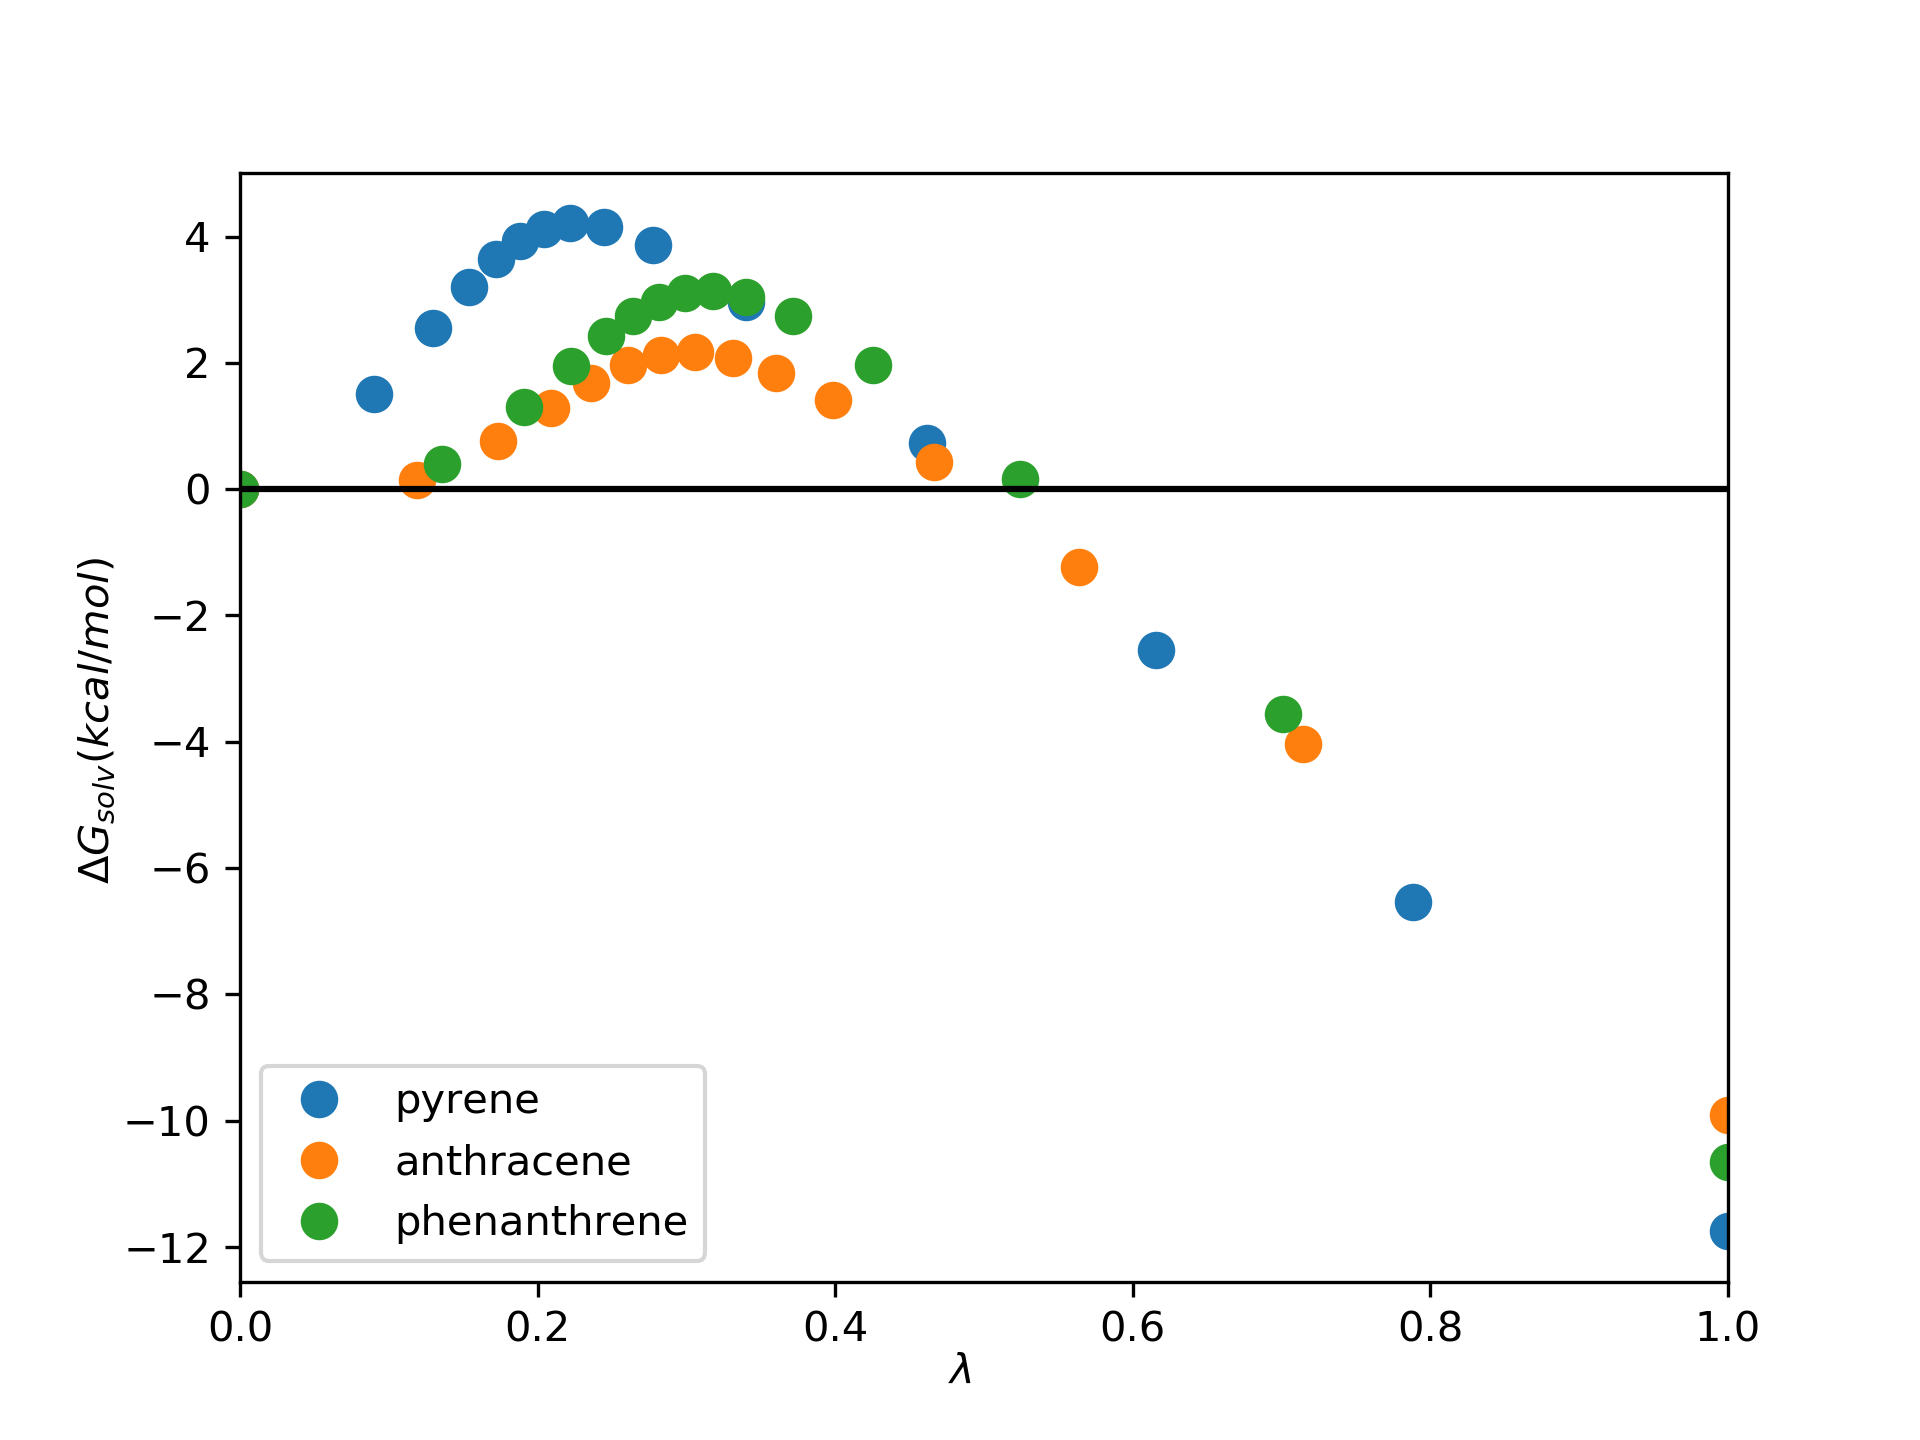
\includegraphics[width=0.8\linewidth]{Figures/tol}
	\caption{Representation of solvation free energies of different solutes in toluene corresponding to each alchemical state. }
	\label{fig:tol}
\end{figure}

The results also indicate a reasonable capability of the force field for predicting the solvation free energies of polyaromatic solutes in aromatic solvents. The influence of the molecular geometry on the solvation free energy curves was the same as the one observed for other solvents, as can be seen in Figure \ref{fig:tol}.  We also calculated the $\Delta G_{solv}$ for phenanthrene in pure toluene and in toluene+$CO_{2}$ mixtures. To the best of our knowledge, there are no available experimental data for these solvation free energies, but the previous results for phenanthrene in other solvents showed that the force field is adequate to describe the solvation phenomenon of phenanthrene in a pure aromatic solvent. Hence, we decided to carry out a qualitative study of the influence of $CO_{2}$ in the solvation free energies of phenanthrene in toluene in order to evaluate the description of this system with the SAFT-$\gamma$ Mie force field. The results for these sets are exposed in Table \ref{tbl:solvco2}.  

\FloatBarrier
\begin{table}[H]
	\centering
	\caption{Calculated values for the solvation free energies (kcal/mol) of phenanthrene in toluene+$CO_{2}$.}
	\label{tbl:solvco2}
	\begin{tabular}{cc}
		\hline
		\hline
		$w_{CO_{2}}$ & $\Delta G_{solv}^{Mie}$ \\
		\hline\hline
		0.0    & -10.65 $\pm$ 0.02   \\
		0.087  & -10.73 $\pm$ 0.02   \\
		0.119  & -10.78 $\pm$ 0.02   \\
		0.169  & -10.71 $\pm$ 0.02   \\
		0.289  & -10.69 $\pm$ 0.02   \\
		\hline
		\hline
	\end{tabular}
\end{table}
\FloatBarrier

The increase of the mass fraction of $CO_{2}$ in toluene caused a small effect on the solvation free energies in the range of weight fractions (0.087-0.289) studied in this dissertation. First, the $\Delta G_{solv}$ decreased with the increase of $w_{CO_{2}}$ up to 0.119. After this, the effect was reversed, and carbon dioxide became an anti-solvent. \citeonline{SOROUSH2014405} reported that asphaltene precipitation occurs when carbon dioxide mass fractions became higher than 0.10 in the system asphaltene+toluene+carbon dioxide, which is in agreement with the anti-solvent effect of carbon dioxide observed in the values calculated here. In the Figure \ref{fig:Figure_1}, we present the free energy profiles of the solvation free energies in the toluene + $CO_{2}$ mixtures. Although we noticed the anti-solvent effect, the differences observed are pretty small. These minor differences may indicate that the effect of $CO_{2}$ is negligible in the solvation of phenanthrene in toluene when using the SAFT-$\gamma$ Mie force field to model the molecules. Nevertheless, more studies need to be done to make a safe assertion about it. It is also worth remarking that this is a qualitative study due to the lack of experimental data. Overall, the methodology proposed by the SAFT-$\gamma$ Mie force field was satisfactory in predicting the solvation free energies of the pairs solvent-solute studied here. For the pair 1-octanol+anthracene, the performance obtained was not as good as it was for the other pairs. This result highlights the importance of choosing a correct geometry for this coarse-grained force field.    

\begin{figure}[H]
	\centering
	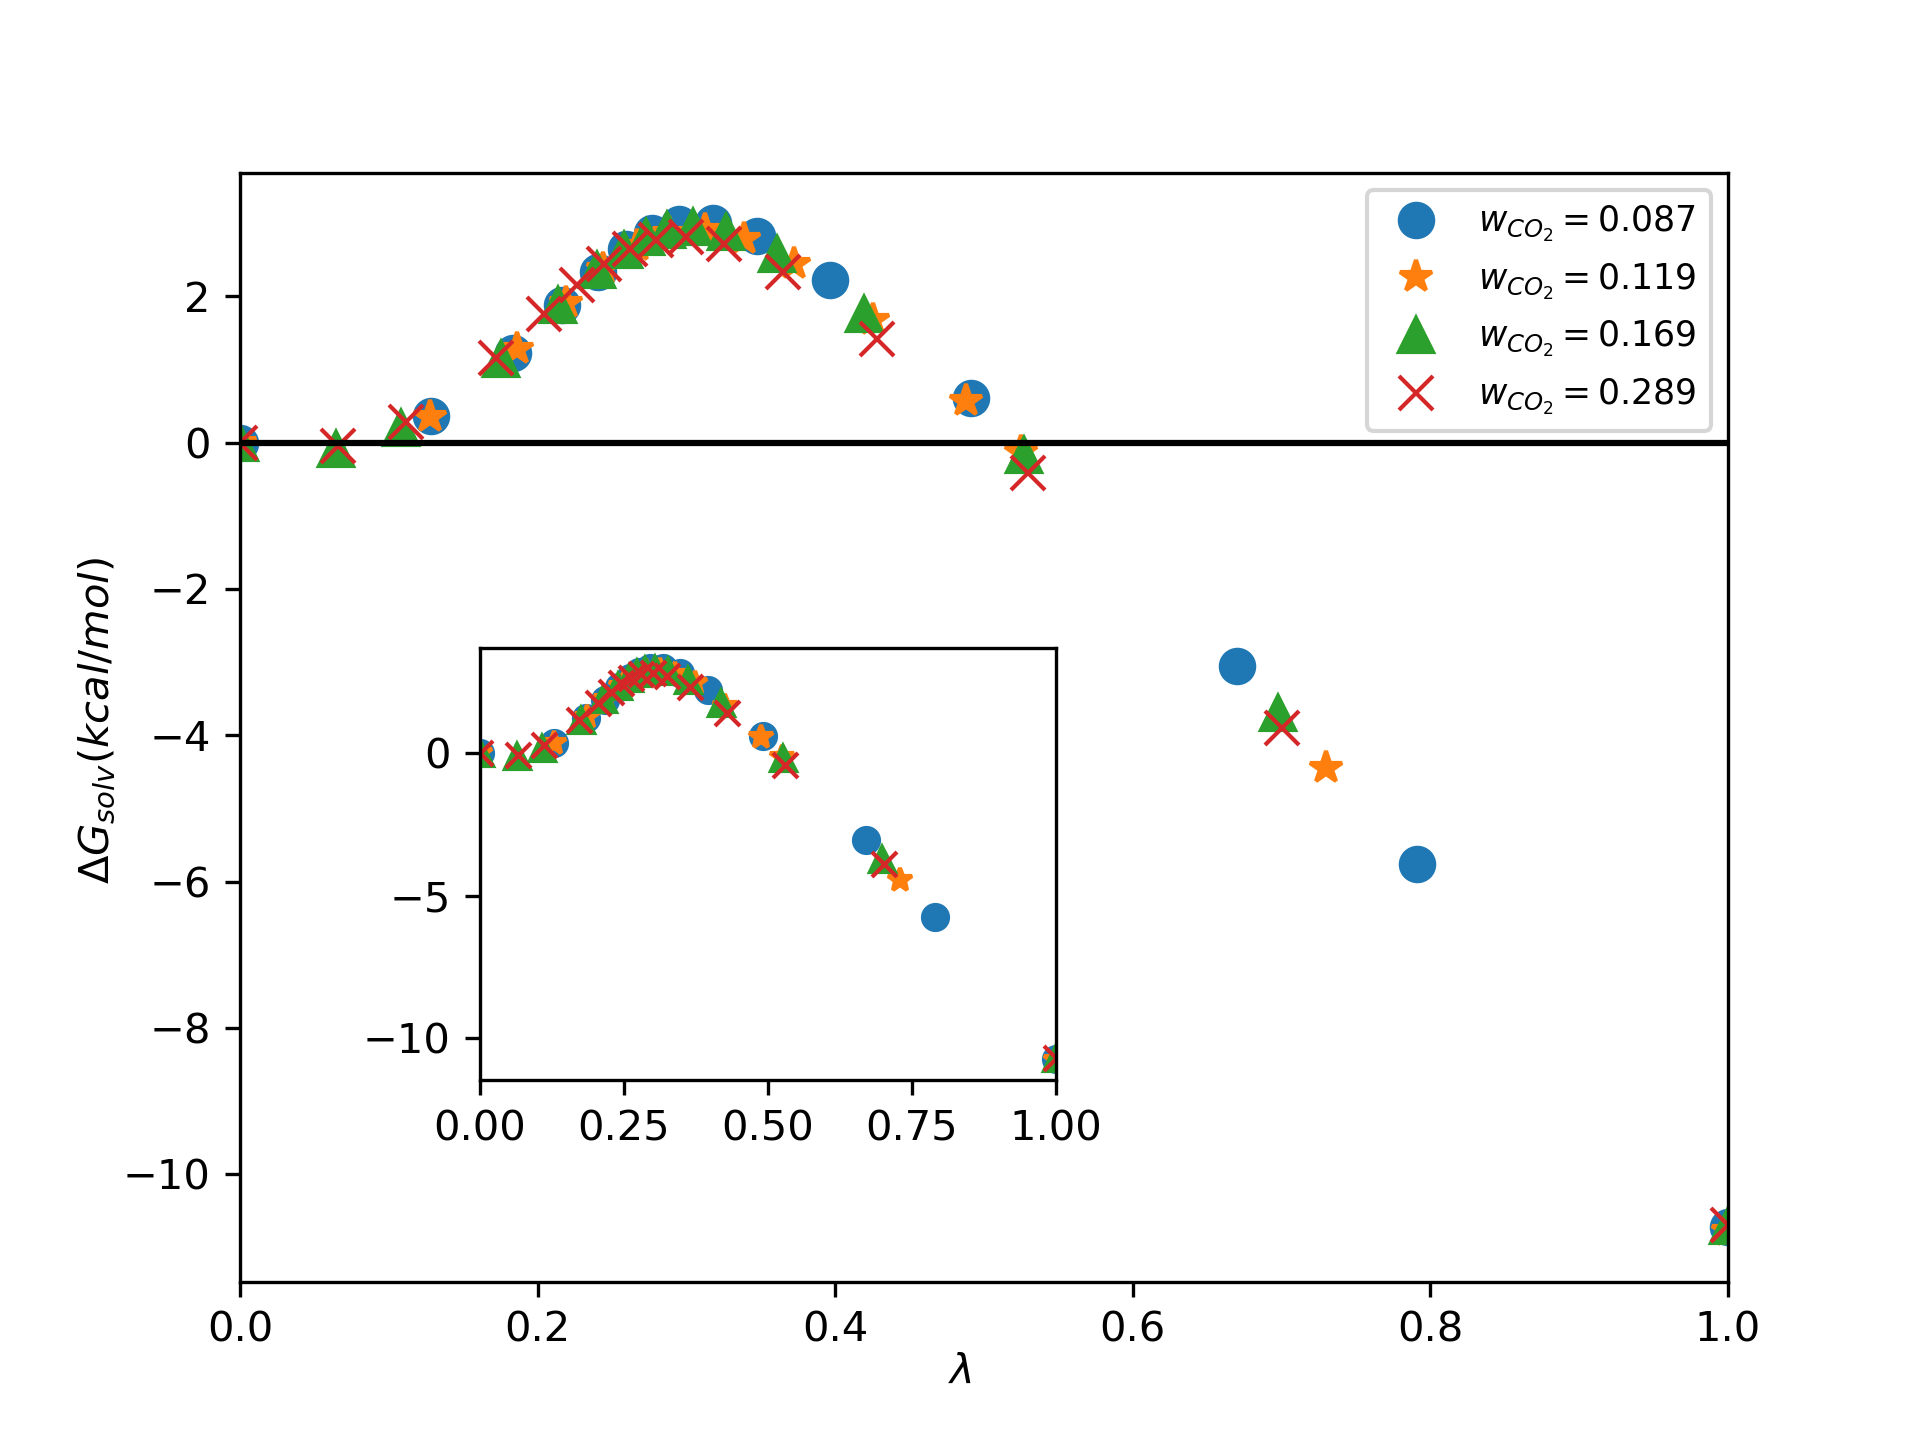
\includegraphics[width=0.8\linewidth]{Figures/tolco2}
	\caption{Representation of solvation free energies of phenanthrene in toluene+$CO_{2}$ corresponding to each alchemical state.}
	\label{fig:Figure_1}
\end{figure}


\section{Hydration free energies}

Water is a solvent extensively used in experimental and computational studies. Because of this importance and the fact that water has unique properties, such as density maximum at 277 K and increased diffusivity upon compression, developing an accurate computational model for water is an ongoing quest \cite{hadley2012}. Hence, we also calculated the solvation free energies in water (hydration free energies) with the SAFT-$\gamma$ Mie force field. With these calculations, we intend to verify if this coarse-grained model would represent the water molecule correctly and would be a good alternative to decrease the computational cost of solvation studies with asphaltene models. The simulations with water as a solvent were carried out using widely studied solutes (propane, benzene) and polyaromatic solutes (toluene, phenanthrene) with a set of fifteen intermediate states.  We obtained these sets of $\lambda$ and $\eta$ with the same methodology used to acquire the sets for the solvation free energies with non-aqueous solvents, and they are exposed in Table \ref{tbl:lambdawater}. At first in our simulations, the binary interaction parameters of all aqueous mixtures were set to zero, but preliminary results for hydration free energies, displayed in Table \ref{tbl:solv3},  exhibited a high deviation from experimental data \cite{P29900000291, doi:10.1021/ct050097l}.

\FloatBarrier
\begin{table*}[h]
	\centering
	\caption{Optimized values of $\lambda $ and $\eta $ for the water+solute pairs. }
	\label{tbl:lambdawater}
	\begin{tabular}{cccccccc}
		\hline\hline
		\multicolumn{2}{c}{propane}& \multicolumn{2}{c}{benzene}& \multicolumn{2}{c}{toluene}& \multicolumn{2}{c}{phenanthrene}\\
		\hline\hline
		$\lambda$ & $\eta$ & $\lambda$ & $\eta$  & $\lambda$ & $\eta$  & $\lambda$ & $\eta$ \\ 
		\hline\hline
		0.000    &    0.000    &    0.000    &    0.000    &    0.000    &    0.000    &    0.000    &    0.000    \\
		0.107    &    2.673    &    0.193    &    -0.295    &    0.177    &    0.182    &    0.142    &    -2.462    \\
		0.157    &    4.703    &    0.279    &    1.468    &    0.262    &    2.432    &    0.256    &    0.597    \\
		0.186    &    6.047    &    0.324    &    2.931    &    0.307    &    4.244    &    0.319    &    4.504    \\
		0.210    &    7.148    &    0.357    &    4.168    &    0.336    &    5.552    &    0.358    &    7.762    \\
		0.230    &    8.017    &    0.381    &    5.091    &    0.360    &    6.696    &    0.384    &    10.104    \\
		0.250    &    8.883    &    0.405    &    5.891    &    0.380    &    7.558    &    0.407    &    12.185    \\
		0.272    &    9.291    &    0.427    &    6.443    &    0.400    &    8.233    &    0.427    &    13.607    \\
		0.294    &    9.700    &    0.449    &    6.770    &    0.422    &    8.678    &    0.446    &    14.490    \\
		0.328    &    9.900    &    0.476    &    6.900    &    0.443    &    8.859    &    0.469    &    14.834    \\
		0.381    &    9.930    &    0.506    &    6.805    &    0.473    &    8.810    &    0.494    &    14.667    \\
		0.484    &    9.463    &    0.555    &    6.392    &    0.514    &    8.452    &    0.533    &    13.832    \\
		0.623    &    8.195    &    0.653    &    5.109    &    0.606    &    7.148    &    0.620    &    11.069    \\
		0.781    &    6.378    &    0.810    &    2.421    &    0.755    &    4.273    &    0.806    &    3.279    \\
		1.000    &    3.333    &    1.000    &    -1.480    &    1.000    &    -1.547    &    1.000    &    -6.122    \\        
		\hline\hline
	\end{tabular}
\end{table*}

\begin{table*}[h]
	\centering
	\caption{Calculated values using $k_{ij}=0$ and experimental values for the hydration free energies (kcal/mol) of solutes in water.}
	\label{tbl:solv3}
	\begin{tabular}{cccc}
		\hline\hline
		Solute       & $\Delta G_{solv}^{exp}$ & $\Delta G_{solv}^{Mie}$ & Absolute Deviation \\ \hline\hline
		propane      & $\,$ 2.00 $\pm$ 0.20         & $\,$ 1.10 $\,$ $\pm$ 0.01         & 0.90               \\
		benzene      & -0.86 $\pm$ 0.20        & -4.45 $\, \,$ $\pm$ 0.03        & 3.59               \\
		toluene      & -0.83 $\pm$ 0.20        & -10.98 $\pm$ 0.30       & 10.15              \\
		phenanthrene & -3.88 $\pm$ 0.60        & -10.90 $\pm$ 0.04       & 7.02               \\ \hline\hline
	\end{tabular}
\end{table*}
\FloatBarrier

With these results, the need for binary interaction parameters became clear. First, we estimated $k_{ij}$ with the SAFT-VR Mie EoS and experimental vapor pressure data, but this strategy also provided results that had high absolute deviations from the experimental data. Therefore, we used the approach of estimating $k_{ij}$ with the output from solvation free energy calculations with molecular dynamics, as described in the last paragraph of Section \ref{solvme}.  We initially found individual values for the interaction parameter of each pair, but, since the parameters for aromatic solutes were very similar (0.148, 0.162, 0.152), we averaged these values. By doing that,  we obtained a general parameter for the water+aromatic pairs, which is exposed in Table \ref{tbl:kij}. Also in this table, we display the binary interaction parameter for the pair water+propane. 

\begin{table*}[h]
	\centering
	\caption{Binary interaction parameters employed.}
	\label{tbl:kij}
	\begin{tabular}{cc}
		\hline
		\hline
		Pair & $k_{ij}$ \\
		\hline\hline
		water+propane      & 0.067  \\
		water+aromatic      & 0.154 \\  
		\hline
		\hline
	\end{tabular}
\end{table*}

The relatively large $k_{ij}$ value of the interaction between aromatic solutes and water can be related to the lack of an explicit association term in the equation of state used to obtain the parameters for water. Actually, the SAFT-VR Mie has an association term \cite{lafitte2013}, but it was not incorporated in the force field. The SAFT-$\gamma$ Mie model for water \cite{lobanova2016} has two different temperature-dependent sets of parameters. The parameters utilized in this work were those estimated with experimental interfacial tension data. Hence, we tested the only binary interaction parameter for water+toluene estimated with MD interfacial data available in the literature \cite{herdes2017}. Nevertheless, the result also had a high absolute deviation, and this parameter could not be transferred to the calculation of the solvation free energy of toluene in water. 

These issues faced by SAFT-$\gamma$ Mie model can also be related to the problems of modeling water with a coarse-grained force field. One of the main difficulties is the choice of which water molecules are going to be represented by which specific beads since water molecules move independently and interact by non-bonded interactions \cite{hadley2010,hadley2012}. The  SAFT-$\gamma$ Mie water considers that one water molecule corresponds to one bead. This strategy only saves a small amount of simulation time, but it can predict properties at physiological temperatures unlike other more aggressive models such as the MARTINI, which considers that one bead represents various water molecules. In light of all these problems related to modeling the water molecule, the SAFT-$\gamma$ Mie force field appears to be a good alternative when working close to room temperatures, but the necessity of additional parameters estimated with molecular simulation indicates severe flaws in the methodology. This estimation of the binary parameter increased significantly the simulation time required to calculate the hydration free energies, since we had to carry out three additional simulations for every pair water-solute and then three other simulations for the three water+polyaromatic solutes in order to test the averaged binary interaction parameter. If these simulations are necessary for every time a new mixture with water is going to be studied with the SAFT-$\gamma$ Mie force field, the use of this model can become impractical.  With this idea in mind, a useful investigation to be made is to check how accurate would be the prediction of the hydration free energy of other aromatic solutes by the SAFT-$\gamma$ Mie force field with the binary interaction parameter estimated here. Using these binary interaction parameters calculated with data from molecular dynamics, we then obtained the final hydration free energies presented in Table \ref{tbl:solv2}. 

\begin{table}[H]
	\centering
	\caption{Calculated and experimental hydration free energies  (kcal/mol) of solutes in water.}
	\label{tbl:solv2}
	\begin{tabular}{cccccc}
		\hline\hline
		Solute       & $\Delta G_{solv}^{GAFF}$ & $\Delta G_{solv}^{ELBA}$ & $\Delta G_{solv}^{exp}$ & $\Delta G_{solv}^{Mie}$ & Absolute  \\
		&                          &                          &                         &                         & Deviation \\ \hline\hline
		propane      & 2.50 $\, \pm$0.02           & 2.76 $\, \pm$ 0.02          & 2.00 $\, \pm$ 0.20         & 2.01 $ \, \pm$ 0.01         & 0.01      \\
		benzene      & -0.81$\pm$0.02           & -0.69 $\pm$ 0.01         & -0.86 $\pm$ 0.20        & -1.12 $\pm$ 0.01        & 0.26      \\
		toluene      & -0.79$\pm$0.03           & -0.76 $\pm$ 0.01         & -0.83 $\pm$ 0.20        & -0.84 $\pm$ 0.01        & 0.01      \\
		phenanthrene & -5.26$\pm$0.03           & N/A                        & -3.88 $\pm$ 0.60        & -3.47 $\pm$ 0.02        & 0.41      \\ \hline\hline
		%    RMSE    &                          &                          & 0.24                    &  \\
		%    \hline  &
	\end{tabular}
	
\end{table}

Hydration free energies calculated using the SAFT-$\gamma$ Mie force field with $k_{ij} \neq 0$ had low absolute deviations from the experimental data, as expected since the parameters were adjusted to fit these experimental data. In the table above, we also show the results obtained by \citeonline{doi:10.1021/acs.jctc.5b00963} with the ELBA force field and by \citeonline{PMID:24928188} with the GAFF force field for the solutes and with the TIP3P model for water. The GAFF (General Amber Force Field) force field is an all-atom model that consists of bonded and non-bonded parameters and is suitable for the study of a significant number of molecules. In turn, the TIP3P model considers that water is a rigid monomer represented by three interacting sites with non-bonded interactions and Coulombic interactions \cite{doi:10.1063/1.445869}. Both the GAFF and the TIP3P models use the Lennard-Jones potential to calculate the non-bonded interactions. The solvation free energies for the ELBA force field were estimated with thermodynamic integration and the solvation free energies with the GAFF force field were estimated with MBAR.

Comparing the results of the three aforementioned force fields, the root mean square error (RMSE) of all the pairs tested with the SAFT-$\gamma$ Mie model was  0.24, the RMSE for hydration free energies obtained with the GAFF force field was 0.73, and that for the ELBA coarse-grained force field was 0.44. The difference in absolute deviations between the GAFF and SAFT-$\gamma$ Mie force fields is significantly high for phenanthrene, hence the coarse-grained force field with a binary parameter is preferred if the application requires a high level of accuracy. The results also indicated that the SAFT-$\gamma$ Mie model with the binary interaction parameter performed better than the ELBA force field in modeling the solvation phenomenon of the pairs studied in this work, but performed worse with the binary parameter set to zero. This difference in performance occurred despite the fact that both the SAFT-$\gamma$ Mie and ELBA models have the same level of coarse-graining for the solvent (one bead represents one water molecule). Therefore, the choice between the two coarse-grained models is dependent on the availability and transferability of binary interaction parameters of the Mie Model. We also present, for the SAFT-$\gamma$ Mie force field, the hydration free energy profiles in Figure \ref{fig:water}. Bigger molecules had steeper free energy profiles, as it was for the solvation free energy study in other solvents. We also observe that the hydration free energy for the first non-zero $\lambda$ is negative for benzene and toluene when a positive value is expected since free energy is required for cavity formation in the solvent for the insertion of the solute. This anomaly can be caused by the fact that the exponential parameters in the Mie potential compensate for cavity formation. 

\begin{figure}[H]
	\centering
	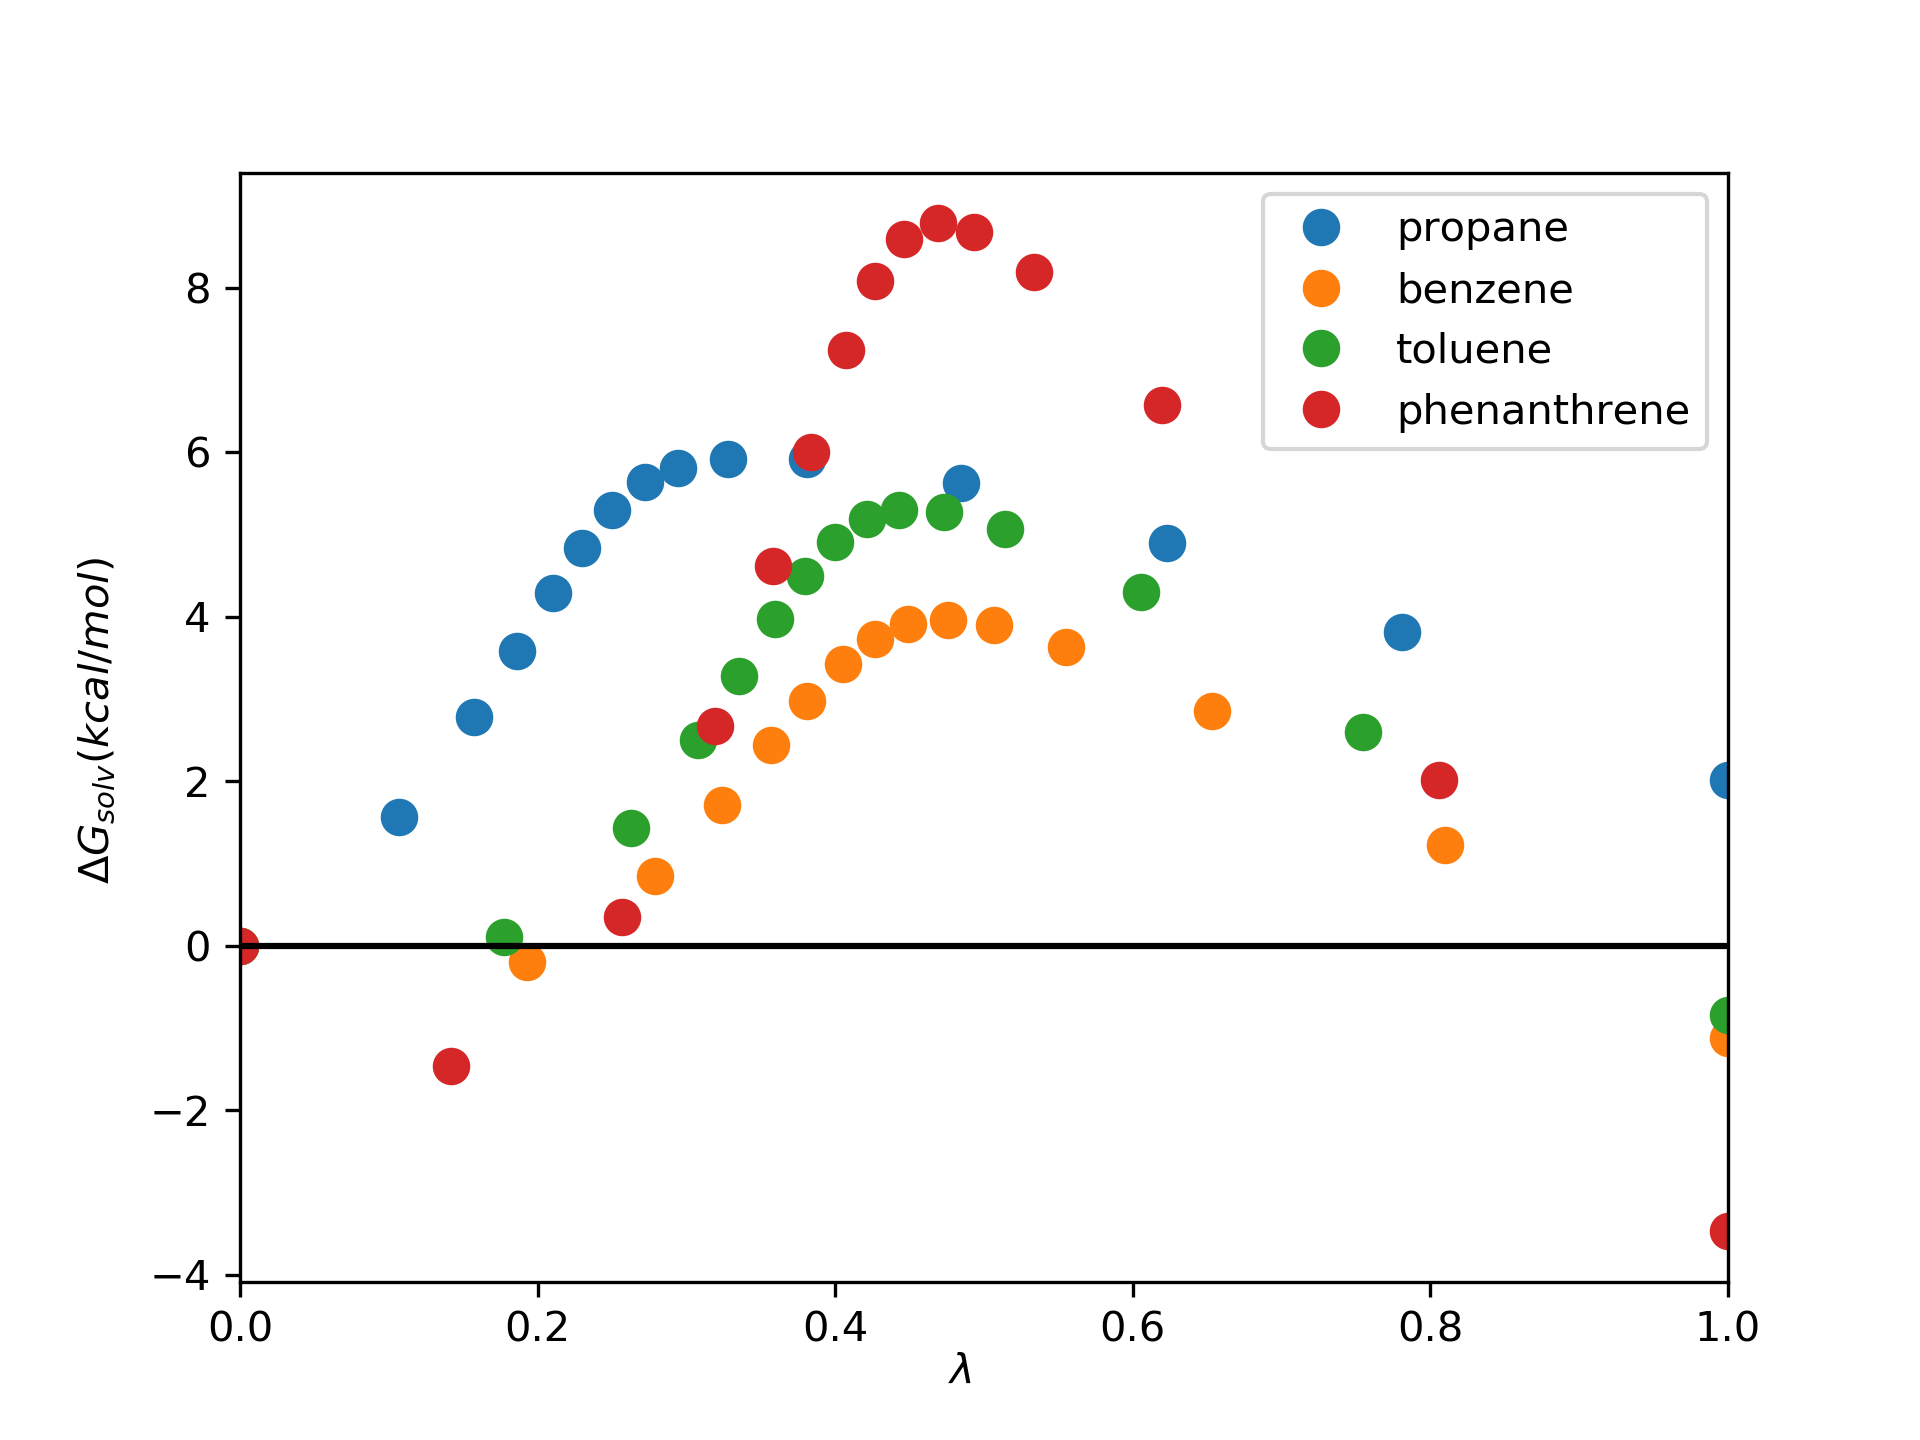
\includegraphics[width=0.8\textwidth]{Figures/water}
	\caption{Representation of hydration free energies of different solutes corresponding to each alchemical state.}
	\label{fig:water}
\end{figure}

The results found here for both the solvation free energies and hydration free energies fulfilled the intentions of this dissertation. We assessed the prediction capability of the SAFT-$\gamma$ Mie force field and provided satisfactory solvation free energy estimates of PAHs using a coarse-grained force field. In addition to that, we found flaws in the methodology used by the SAFT-$\gamma$ Mie force field to model the water molecule. Hence, these shortcomings of this model can now be addressed, and the force field can even be improved by using other mixing rules to avoid the use of a binary parameter or, even, using hydration free energy estimates in the parameterization of water. These results also encourage us to calculate solvation free energies of more complex molecules mimicking asphaltenes in non-aqueous solvents in future studies.  

\section{Partition Coefficients}

Using the solvation free energies estimated in the sections above, we also calculated partition coefficients by means of Eq. \eqref{eqn:partcoe}, for the pairs  water/1-octanol and water/hexane with the intention of testing the modeling capabilities of the SAFT-$\gamma$ Mie force field again. The partition functions studied here have many experimental data available in the literature due to their environmental importance \cite{sangster}. Besides this, the calculations of these specific partition coefficients are relevant because   1-octanol is used to quantify hydrophobicity and can serve as a model for biological lipids and different soils \cite{RUELLE2000457}, and hexane is a model for an apolar, hydrophobic phase. Calculated values and experimental data are shown in Table \ref{tbl:part}. The experimental data of the partition coefficients were taken from   \citeonline{POOLE2000117,sangster} for the coefficient of water/1-octanol and from \citeonline{doi:10.1021/je970112e} for the coefficient of water/hexane. 

\begin{table}[H]
	\centering
	\caption{Partition Coefficient Calculated from MD simulations and from experimental data.}
	\label{tbl:part}
	\begin{tabular}{cccc}
		\hline\hline
		& {Molecular Dynamics} & {Experimental} & Absolute Deviation \\ \hline
		\multicolumn{4}{c}{log $P^{water/1-octanol}$}               \\ \hline
		propane      & 2.47                 & 2.40           & 0.07               \\
		phenanthrene & 3.57                 & 4.46           & 0.89               \\ \hline
		\multicolumn{4}{c}{log $P^{water/hexane}$}                 \\ \hline
		benzene      & 1.93                 & 2.06           & 0.13               \\
		phenanthrene & 4.17                 & 4.49           & 0.32               \\
		%                       \multicolumn{4}{c}{log $P^{tolune/hexane}$}                \\ \hline
		%        pyrene       & -0.67                & -0.97          & 0.30               \\
		%        phenanthrene & -0.47                & -              & -                  \\ 
		\hline\hline
	\end{tabular}
	
\end{table}

Overall absolute deviations were small for pairs with smaller solvation free energy deviations such as propane and benzene. The water/1-octanol partition coefficient of phenanthrene had higher deviation due to the higher deviation of the free energy of solvation of this compound in 1-octanol. Comparing with other force fields, \citeonline{garrido} reported average absolute deviations for the water/1-octanol partition coefficient of 0.4 with the GROMOS 53a6 force field \cite{JCC:JCC20090}, 0.3 for TraPPE, and 0.9 for OPLS-AA/TraPPE force fields. However, they attribute the low deviations of TraPPE to the cancellation of errors between the two solvation free energies. Additionally, \citeonline{doi:10.1021/acs.jctc.5b00963} found average absolute deviations of 0.86 for the water/hexane partition coefficients and of 0.75 for the water/1-octanol partition coefficients with the ELBA coarse-grained force field. In this dissertation, we performed a small study of partition coefficients with the SAFT-$\gamma$ Mie force field. Hence, a larger set would be necessary to do a complete evaluation of the performance of this force field in the prediction of partition coefficients. 